\section{Evaluation}
\label{sec:evaluation}

\subsection{Multicollinearity}
\label{sec:multicollinearity}
Multicollinearity among the regressor variables was checked and those with high variable inflation factor or VIF were removed. The VIF of a variable is the ratio of the variance of the overall model to the variance of a model with only that variable. A VIF greater than 4 indicates moderate multicollinearity and a VIF greater than 10 indicates severe multicollinearity. The regressor variables of Hepatitis.B, transformed logGDP, logPopulation, thinness.5.9.years, Income.composition.of.resources, and, Schooling were removed because these had greater than 4 VIF, and their p-value in the model summary indicated lower significance. 
After removing these variables, the model was fitted and again the VIF and the Pearson correlation coefficients for the variables were calculated. The regressor variables: log_under.five.deaths, and log_infant.deaths again had very high VIF and these were taken care of later while considering the interactions between the regressors.

\subsection{Identification of Influential Points}
\label{sec:influential-points}
Further, the points that play an important role than others in determining the regression line were found. High leverage points were looked for by finding fitted values that were greater than 2* (k+1)/n, where k is the number of variables in the model and n is the number of observations used to create the model. The outliers were searched by identifying where the absolute internally studentized and externally studentized residuals are greater than 3. Then, three methods were used to identify potentially influential points. The first method that was used is Difference in Fits, or DFFITS, which is a measure of the difference in fitted values when a chosen observation is removed from the model. A point was considered influential if the absolute value of $DFFITS_i$ was greater than $2* \sqrt{(k+2)/(n-k-2)}$. The second method that was used was Cook’s distance, $D_i$, which identifies influential points by determining which observations had high leverage or were outliers. An observation was considered possibly influential if the value returned from the R function: \textit{cooks.distance()} was greater than 1. The third method used was COVRATIO. An observation was considered possibly influential if the value of $COVRATIO_i$ was greater than $1+ 3*((k+1)/n)$, or less than $1- 3*((k+1)/n)$.
About 7\% of the data points were removed that were overlapping in influential, high leverage, and outlier observations.

\section{Assumptions of a Linear model}
\label{sec:assumptions}

\subsection{Linearity between Explanatory and Response variables}
\label{sec:linearity}
As can be seen from the plots of residual errors again the regressor variables shown in the figure \ref{fig:linearity}, there is not much of a pattern and they are mostly scattered. If these plots are scanned from left to right by considering thin vertical strips, in each strip, the vertical average of the residuals is mostly zero except for Alcohol and Adult mortality. So the assumption about the linearity of our model is satisfied. 

\begin{figure}
  \centering
  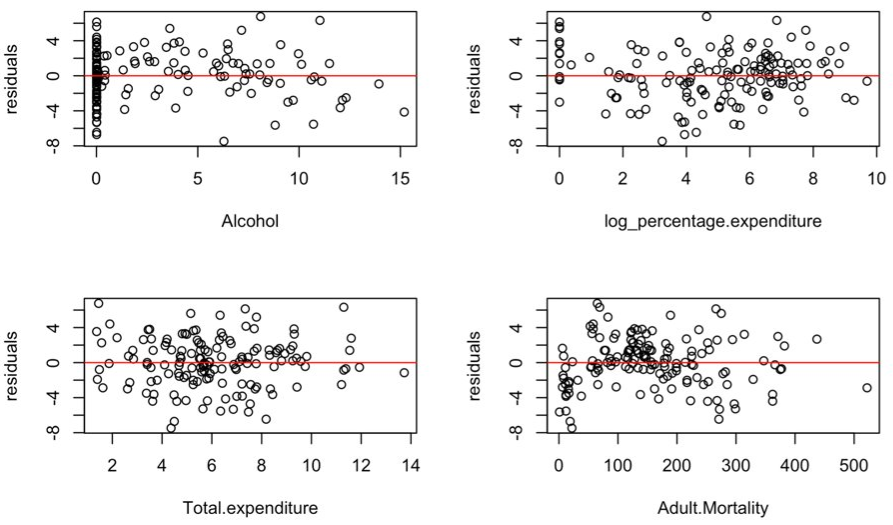
\includegraphics[width = 0.9\textwidth]{figures/linearity.PNG}
  \caption{Residual errors against the regressors}
  \label{fig:linearity}
\end{figure}

\subsection{Independence of Error Terms}
\label{sec:independence}
In the figure \ref{fig:independence}, the residual errors are plotted against the row numbers sorted by regressor variables for checking the independence of error terms assumption. As these plots are scanned from left to right by considering thin vertical strips, it is noticed that they are randomly and symmetrically distributed around zero. Hence, it is concluded that our model passed the assumption of independence of error terms. 

\begin{figure}
  \centering
  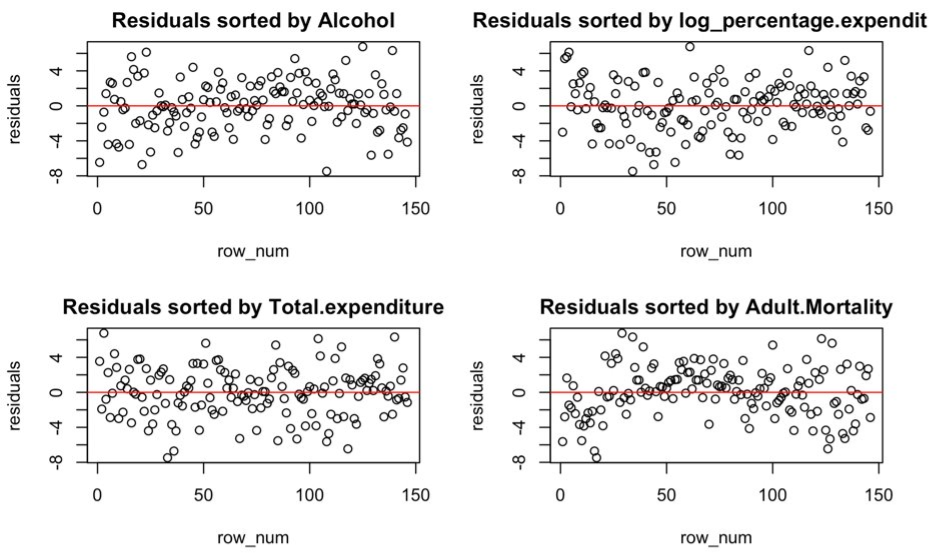
\includegraphics[width = 0.9\textwidth]{figures/independence.PNG}
  \caption{Residuals against the row numbers sorted by regressors}
  \label{fig:independence}
\end{figure}

\subsection{Normality in the Distribution of Error Terms}
\label{sec:normality}
As can be seen from the figure \ref{fig:normality} showing the Q-Q plot, the points approximately fall on a straight line, which supports the assumption of normality between error terms.

\begin{figure}
  \centering
  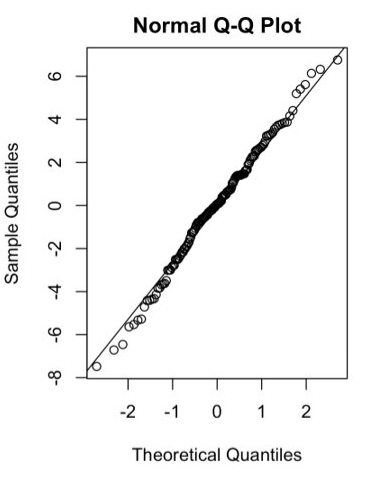
\includegraphics[width = 0.9\textwidth]{figures/normality.PNG}
  \caption{Normal Q-Q plot}
  \label{fig:normality}
\end{figure} 

The Shapiro-Wilk test was also conducted to check for the normal distribution of the error terms where the null hypothesis is that the errors follow a normal distribution. As shown in the figure \ref{fig:shapiro}The p-value obtained from the test was 0.77 which is greater than the \textit{alpha} of 0.05. Hence, we failed to reject the null hypothesis and thus it was found that the error terms follow the normal distribution. 

\begin{figure}
  \centering
  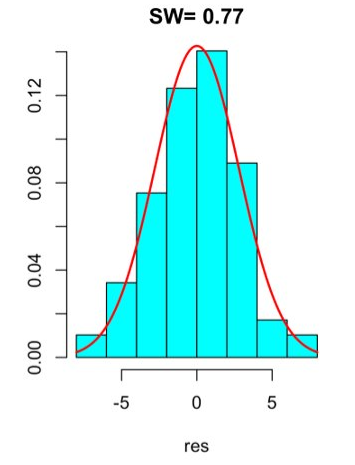
\includegraphics[width = 0.9\textwidth]{figures/Shapiro.PNG}
  \caption{Plot for error terms with p-value from Shapiro-Wilk test}
  \label{fig:shapiro}
\end{figure}



%%% Local Variables:
%%% TeX-master: "main"
%%% End:
